\documentclass[conference]{IEEEtran}
\usepackage{amsmath,amssymb}
\usepackage{graphicx}
\usepackage{booktabs}
\usepackage{xcolor}
\usepackage{tikz}
\usetikzlibrary{positioning,arrows.meta}
\usepackage{cite}
\usepackage{url}

% Red text = something the team must fill in or confirm before submitting.
\newcommand{\fillin}[1]{\textcolor{red}{[#1]}}

\begin{document}

\title{Re-implementing Harmonic--Percussive\\Time-Scale Modification of Music in MATLAB}

\author{
\IEEEauthorblockN{Anshika \fillin{Surname}, Mridhula \fillin{Surname}, Anya Maheshwari}
\IEEEauthorblockA{Department of Electrical and Communication Engineering, Shiv Nadar University\\
ECE 2003 Signal Representation and Processing, Monsoon 2026}
}

\maketitle

\begin{abstract}
Time-scale modification (TSM) changes the tempo of an audio signal without changing its pitch. Classic TSM algorithms degrade percussive transients: the phase vocoder smears them, while time-domain methods make them stutter. Driedger, M\"uller and Ewert proposed avoiding explicit transient detection by first separating the signal into a harmonic and a percussive component, stretching the harmonic part with a phase vocoder and the percussive part with plain overlap-add (OLA) using very short frames, and adding the results. We re-implement this method from first principles in MATLAB, together with the phase vocoder and WSOLA as baselines, and verify every block with unit tests. On a synthetic test signal of tones and clicks, the combined method reproduces the input to within $4\times10^{-12}$ at unit stretch, preserves pitch exactly, places every click at its scaled time, and keeps clicks as sharp as in the original (sharpness 0.84 versus 0.84), whereas the phase vocoder smears them (0.52) and WSOLA doubles three of seven. We also report results on real music and discuss where the method fails.
\end{abstract}

\begin{IEEEkeywords}
Time-scale modification, harmonic-percussive separation, phase vocoder, overlap-add, WSOLA, transient preservation.
\end{IEEEkeywords}

%======================================================================
\section{Introduction}

Stretching music in time while keeping its pitch is needed in music practice, DJ beat-matching and fitting audio to video. Simply resampling a signal changes its pitch, so TSM algorithms instead cut the signal into short overlapping frames and re-space them. Two standard approaches are the phase vocoder (PV)~\cite{flanagan66}, which works in the frequency domain with long frames, and time-domain overlap-add methods such as WSOLA~\cite{verhelst93}. Both handle sustained tones reasonably well but degrade percussive transients such as drum hits: the PV smears them in time, and WSOLA tends to repeat them.

Several methods detect transients explicitly and treat them separately~\cite{nagel09}, but detection errors then directly damage the output. Driedger \emph{et al.}~\cite{driedger14} proposed a simpler idea: separate the signal into a harmonic component $x_h$ and a percussive component $x_p$ with median filtering~\cite{fitzgerald10}, stretch $x_h$ with a PV using long frames and $x_p$ with plain OLA using very short frames, and add the results (Fig.~\ref{fig:pipeline}). No transient detector is needed.

In this project we re-implement that method in MATLAB from our own STFT upward, build the PV and WSOLA baselines, and test each block against precise acceptance criteria before integrating them. Section~\ref{sec:background} reviews the building blocks, Section~\ref{sec:method} describes the method, Section~\ref{sec:impl} our implementation, Section~\ref{sec:results} the results, and Section~\ref{sec:discussion} the limitations.

\begin{figure}[t]
\centering
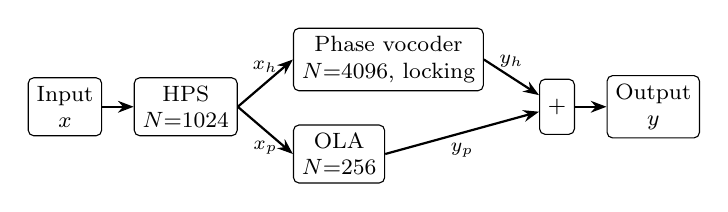
\begin{tikzpicture}[
  node distance=4mm and 4mm,
  blk/.style={draw, rounded corners=2pt, align=center, font=\footnotesize, minimum height=7mm, inner sep=3pt},
  ar/.style={-{Stealth[length=2mm]}, thick}]
\node[blk] (x) {Input\\$x$};
\node[blk, right=of x] (hps) {HPS\\$N{=}1024$};
\node[blk, right=7mm of hps, yshift=6mm] (pv) {Phase vocoder\\$N{=}4096$, locking};
\node[blk, right=7mm of hps, yshift=-6mm] (ola) {OLA\\$N{=}256$};
\node[blk, right=7mm of pv, yshift=-6mm] (sum) {$+$};
\node[blk, right=of sum] (y) {Output\\$y$};
\draw[ar] (x) -- (hps);
\draw[ar] (hps.east) -- node[above, font=\scriptsize]{$x_h$} (pv.west);
\draw[ar] (hps.east) -- node[below, font=\scriptsize]{$x_p$} (ola.west);
\draw[ar] (pv.east) -- node[above, font=\scriptsize]{$y_h$} (sum);
\draw[ar] (ola.east) -- node[below, font=\scriptsize]{$y_p$} (sum);
\draw[ar] (sum) -- (y);
\end{tikzpicture}
\caption{Harmonic--percussive TSM (HP). The input is split into a harmonic part, stretched with a long-frame phase vocoder, and a percussive part, stretched with short-frame OLA; the two outputs are added.}
\label{fig:pipeline}
\end{figure}

%======================================================================
\section{Background}
\label{sec:background}

\subsection{Short-time Fourier transform}
For a frame size $N$, hop $H$ and window $w$, the STFT of $x$ is
\begin{equation}
X(t,k)=\sum_{n=0}^{N-1} w(n)\,x(n+tH)\,e^{-2\pi i kn/N},
\label{eq:stft}
\end{equation}
with frame index $t$ and frequency bin $k\in[0:N/2]$. We use a periodic Hann window $w(n)=\tfrac12-\tfrac12\cos(2\pi n/N)$ throughout.

\subsection{Overlap-add time-scale modification}
TSM by a factor $\alpha$ takes analysis frames $x_t$ from the input at positions $a_t$, optionally modifies them into $y_t$, and places them $H_s$ samples apart in the output~\cite{driedger14}:
\begin{equation}
y(m)=\frac{\sum_t w(m-tH_s)\,y_t(m-tH_s)}{\sum_t w(m-tH_s)}.
\label{eq:ola}
\end{equation}
Plain OLA uses $y_t=x_t$. Because consecutive frames of a periodic signal no longer line up, OLA introduces phase jumps that make tones sound rough. For noise-like sounds and transients the phase is already random, so these jumps are inaudible, and with very short frames a transient stays at its place and stays crisp~\cite{driedger14}.

\subsection{Phase vocoder}
The PV~\cite{flanagan66} keeps each sinusoid continuous across output frames. From the phase advance of bin $k$ between two analysis frames it estimates the bin's true (instantaneous) frequency and advances the output phase by $H_s$ times that frequency. It needs long frames for frequency resolution, which is exactly why it smears transients: a hit is spread over the whole frame~\cite{laroche99}.

\subsection{WSOLA}
WSOLA~\cite{verhelst93} is OLA in which each analysis frame may move within a tolerance $\pm\Delta$ of its nominal position, to the position whose waveform best continues the previous output frame. This removes most phase jumps for tonal signals, but with long frames a transient can be copied into two neighbouring frames and heard twice.

%======================================================================
\section{Method}
\label{sec:method}

\subsection{Harmonic--percussive separation}
In a magnitude spectrogram $Y=|X|$, a sustained tone is a horizontal line and a percussive hit is a vertical line. Median filtering $Y$ along time removes the short vertical spikes and keeps horizontal structure; median filtering along frequency does the opposite~\cite{fitzgerald10}:
\begin{align}
\tilde Y_h(t,k)&=\operatorname{median}\big(Y(t-\ell,k),\dots,Y(t+\ell,k)\big),\label{eq:medh}\\
\tilde Y_p(t,k)&=\operatorname{median}\big(Y(t,k-\ell),\dots,Y(t,k+\ell)\big).\label{eq:medp}
\end{align}
Binary masks $M_h=(\tilde Y_h\ge\tilde Y_p)$ and $M_p=(\tilde Y_p>\tilde Y_h)$ are applied to the complex STFT, $X_h=X\odot M_h$ and $X_p=X\odot M_p$, and each is inverted with the least-squares inverse STFT of Griffin and Lim~\cite{griffin84}. Since $M_h+M_p=1$ and the inverse STFT is linear, $x_h+x_p=x$ exactly.

\subsection{Phase vocoder with identity phase locking}
Let $\phi(t,k)$ be the analysis phase, $\omega_k=2\pi k/N$ the bin centre frequency and $H_{a,t}=a_t-a_{t-1}$ the actual analysis hop. The phase deviation and instantaneous frequency are
\begin{align}
\Delta\phi&=\operatorname{wrap}\big(\phi(t,k)-\phi(t-1,k)-\omega_k H_{a,t}\big),\\
\hat\omega(t,k)&=\omega_k+\Delta\phi/H_{a,t},
\end{align}
where $\operatorname{wrap}$ maps to $(-\pi,\pi]$. The basic PV sets the output phase to $\phi_y(t,k)=\phi_y(t-1,k)+H_s\,\hat\omega(t,k)$. Treating every bin independently lets the bins around one sinusoid drift apart in phase, which causes ``phasiness''. Identity phase locking~\cite{laroche99} updates the phase only at spectral peaks $p$ (bins at least as large as their two neighbours on each side) and sets every other bin relative to its nearest peak $p(k)$:
\begin{equation}
\phi_y(t,k)=\phi_y\big(t,p(k)\big)+\phi(t,k)-\phi\big(t,p(k)\big).
\end{equation}
Each output frame is the inverse FFT of $|X(t,k)|e^{i\phi_y(t,k)}$, windowed again and overlap-added; because the frame is windowed twice, the output is normalised by $\sum_t w^2(m-tH_s)$ instead of $\sum_t w$, which also compensates the energy loss noted in~\cite{driedger14}.

\subsection{OLA for the percussive part and recombination}
The percussive part is stretched with~\eqref{eq:ola}, $y_t=x_t$ and $N=256$. Both stretched parts are exactly $\operatorname{round}(\alpha L)$ samples long for an input of $L$ samples, so the output is simply $y=y_h+y_p$.

%======================================================================
\section{Implementation}
\label{sec:impl}

All code is plain MATLAB with our own STFT and inverse STFT; no toolbox TSM or STFT functions are used. Audio is converted to mono, resampled to 22\,050~Hz and peak-normalised. The team split the work into three blocks with a fixed interface: \texttt{hps.m} (Anshika), \texttt{tsm\_pv.m} (Mridhula), and \texttt{tsm\_ola.m}, the WSOLA baseline \texttt{tsm\_wsola.m}, integration and experiments (Anya Maheshwari). Table~\ref{tab:params} lists the parameters.

\begin{table}[t]
\centering
\caption{Parameters (sampling rate 22\,050 Hz)}
\label{tab:params}
\begin{tabular}{@{}lccl@{}}
\toprule
Block & $N$ & Hop & Normalisation \\
\midrule
HPS ($\ell=5$) & 1024 & 256 & $\sum w^2$ \\
Phase vocoder & 4096 & $H_s=1024$ & $\sum w^2$ \\
OLA (percussive) & 256 & $H_s=128$ & $\sum w$ \\
WSOLA (baseline) & 1024 & $H_s=512$, $\Delta=256$ & $\sum w$ \\
\bottomrule
\end{tabular}
\end{table}

The frame sizes, median filter length and stretch factors follow~\cite{driedger14}; the hop sizes and WSOLA settings are our choices because the paper does not give them. All three TSM functions share one synthesis recipe: a fixed integer synthesis hop $H_s$ and analysis positions $a_t=\operatorname{round}(tH_s/\alpha)$. Using a fixed analysis hop and rounding $H_s=\alpha H_a$ instead would make the effective stretch differ slightly from $\alpha$ and drift over a long clip. Because $a_t$ is rounded, the PV uses the actual hop $H_{a,t}$ in its phase update, which avoids a slow pitch drift.

Each block was first tested on its own against acceptance tests, then integrated. The test signals are a 4~s tone (A4 for 2~s then E5, with two harmonics), a train of decaying noise bursts every 0.5~s starting at 0.25~s (``clicks''), and their mix.

To measure transient sharpness objectively we high-pass each output with a second difference $d(m)=y(m+1)-2y(m)+y(m-1)$, which suppresses the steady tone, and compute for each click the share of the energy of $d$ in a 100~ms window that falls inside its loudest 10~ms, averaged over all clicks. A crisp click scores close to the original; a smeared or doubled click scores lower.

%======================================================================
\section{Results}
\label{sec:results}

\subsection{Verification of each block}
Table~\ref{tab:verify} summarises the tests. Every function returns exactly $\operatorname{round}(\alpha L)$ samples for $\alpha\in\{0.5,1,1.2,1.8,3\}$, and at $\alpha=1$ every TSM method reproduces its input to numerical precision, which checks framing, windowing and normalisation. The PV keeps the 440~Hz fundamental at every stretch factor, with and without phase locking. Through the full pipeline at $\alpha=1.8$, all seven clicks appear at $1.8$ times their original onset times (0.45~s, 1.35~s, \dots, 5.85~s) to within 1~ms.

\begin{table}[t]
\centering
\caption{Verification on the test signals}
\label{tab:verify}
\begin{tabular}{@{}lr@{}}
\toprule
Test & Result \\
\midrule
HPS: $\max|x_h+x_p-x|$ & $3.3\times10^{-16}$ \\
HPS: tone energy in $x_h$ / click energy in $x_p$ & 99.8\% / 100\% \\
PV identity error at $\alpha=1$ (no lock / lock) & $6.2 / 8.8\times10^{-12}$ \\
PV pitch at $\alpha=1.2, 1.8, 3$ & 440.0 Hz \\
OLA / WSOLA identity error at $\alpha=1$ & $1.1\times10^{-16}$ / $2.2\times10^{-16}$ \\
Full pipeline identity error at $\alpha=1$ & $4.1\times10^{-12}$ \\
Click onsets at $\alpha=1.8$ (full pipeline) & 7 of 7 within 1 ms \\
\bottomrule
\end{tabular}
\end{table}

\subsection{Separation}
Fig.~\ref{fig:hps} shows the separation of the test mix. The harmonic part keeps only the horizontal note lines and the percussive part only the vertical click lines. The sudden note change at 2~s is itself a short broadband event and is partly assigned to the percussive part, as expected.

\begin{figure}[t]
\centering
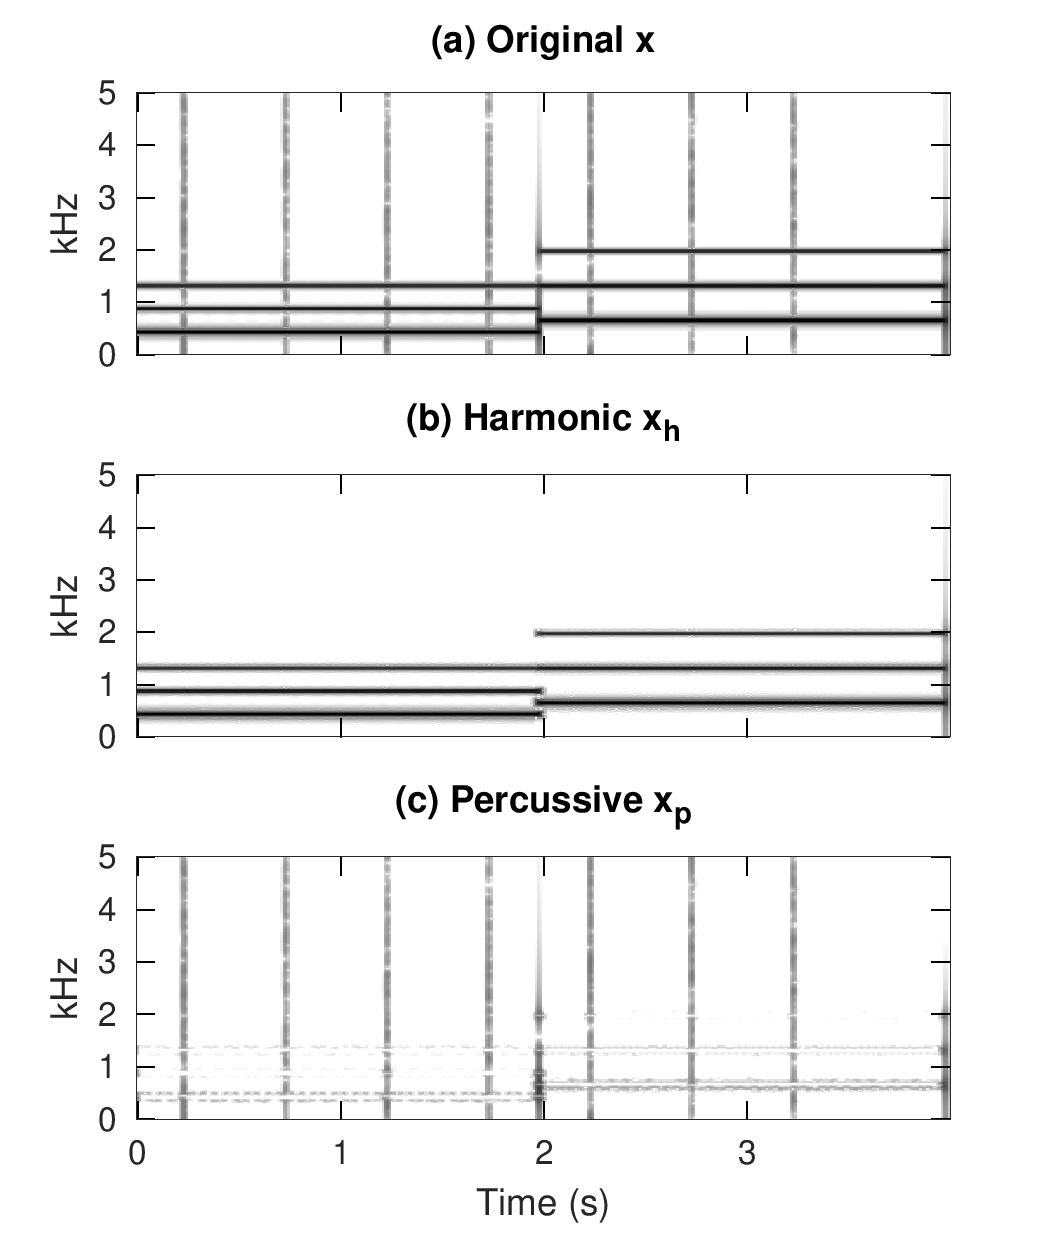
\includegraphics[width=\columnwidth]{fig/hps.png}
\caption{Harmonic--percussive separation of the test mix (spectrograms, common dB scale). (a) Input. (b) Harmonic part: note lines only. (c) Percussive part: clicks only.}
\label{fig:hps}
\end{figure}

\subsection{Why OLA is used only on the percussive part}
On the clicks alone at $\alpha=1.8$, OLA with $N=256$ keeps 96.7\% of each click's energy in its loudest 10~ms (original 99.9\%), but with $N=2048$ only 67.0\%, because long frames copy each click into several overlapping frames. On the pure tone, however, OLA destroys the harmonic structure: 99.96\% of the output energy lies outside $\pm5$~Hz of the three harmonics. WSOLA with $N=1024$ keeps the tone clean (below 0.01\% outside the harmonics, versus 69.2\% for OLA with the same frame size), but doubles three of the seven clicks.

\subsection{Transient preservation}
Fig.~\ref{fig:transient} shows one click of the test mix before and after stretching by 1.8 with each method, high-passed so that the tone drops out. HP reproduces a single sharp click. The PV spreads the click over about 50~ms, WSOLA repeats it three times, and OLA keeps it sharp. Table~\ref{tab:sharp} gives the sharpness measure averaged over all clicks. HP matches the original (0.84), the PV loses about 40\% (0.52), and WSOLA falls in between because of the doubled clicks. OLA scores highest, but only because it destroys the tone (previous subsection). Fig.~\ref{fig:spec} shows the same effect in the spectrogram: in HP the clicks stay thin vertical lines, while in the PV they widen.

\begin{figure}[t]
\centering
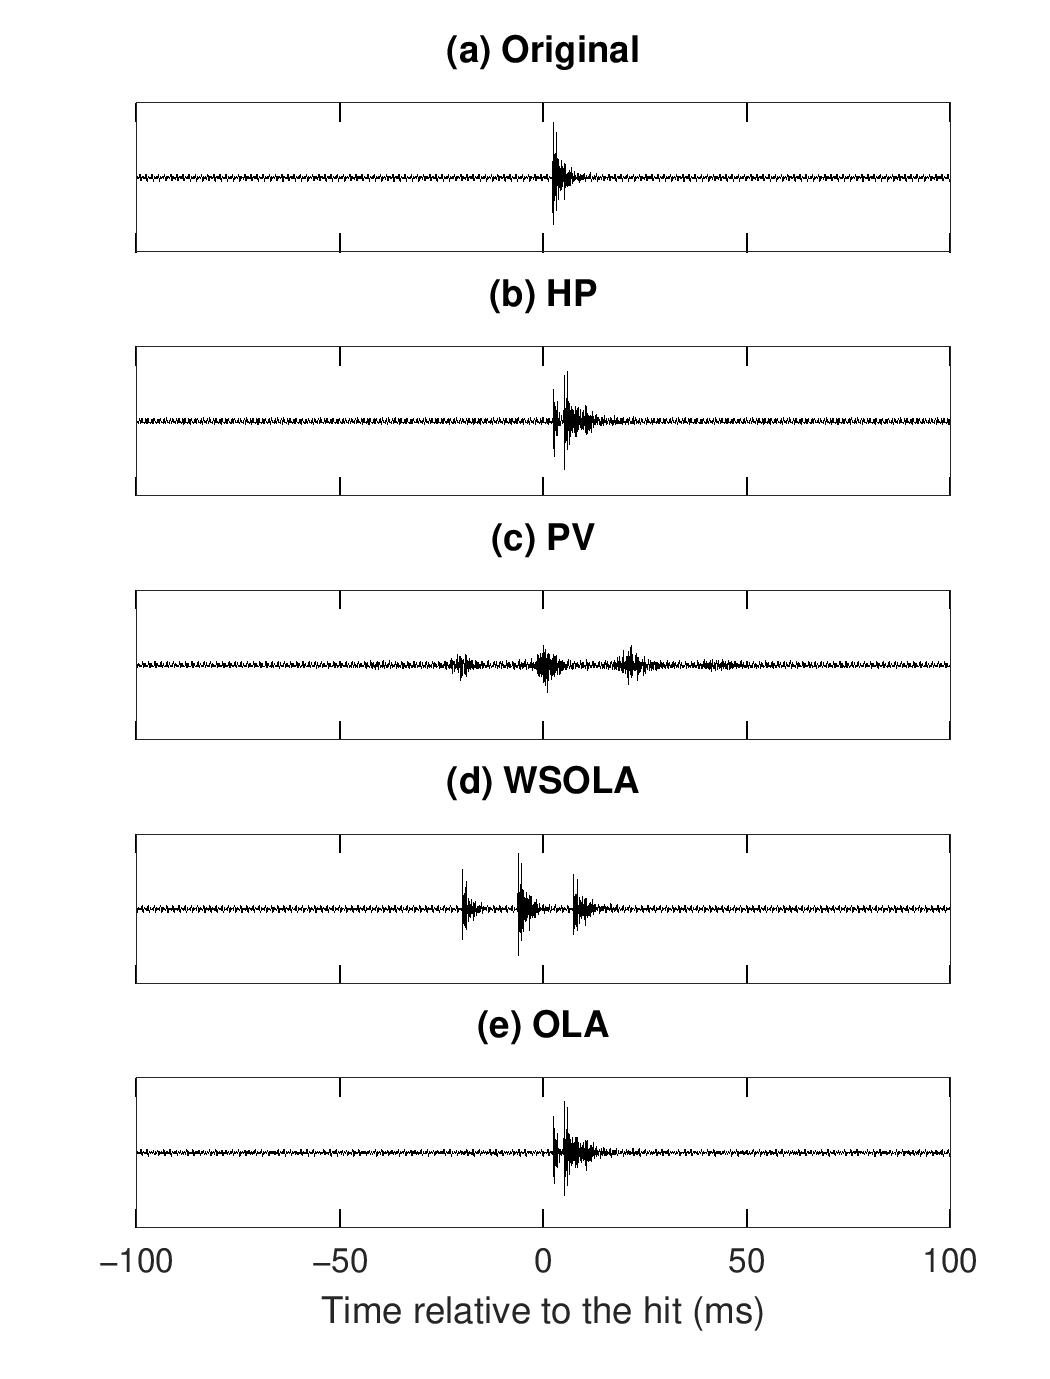
\includegraphics[width=\columnwidth]{fig/transient.png}
\caption{One click of the test mix (at 2.25~s), high-passed, $\pm100$~ms around the hit. (a) Original. (b)--(e) Stretched by $\alpha=1.8$ with HP, PV, WSOLA and OLA, aligned at the scaled hit time. Compare with Fig.~3 of~\cite{driedger14}.}
\label{fig:transient}
\end{figure}

\begin{table}[t]
\centering
\caption{Click sharpness on the test mix, $\alpha=1.8$}
\label{tab:sharp}
\begin{tabular}{@{}lcl@{}}
\toprule
Method & Sharpness & Note \\
\midrule
Original & 0.84 & reference \\
\textbf{HP} & \textbf{0.84} & tone clean \\
PV & 0.52 & clicks smeared \\
WSOLA & 0.80 & some clicks doubled \\
OLA (whole signal) & 0.87 & tone destroyed \\
\bottomrule
\end{tabular}
\end{table}

\begin{figure}[t]
\centering
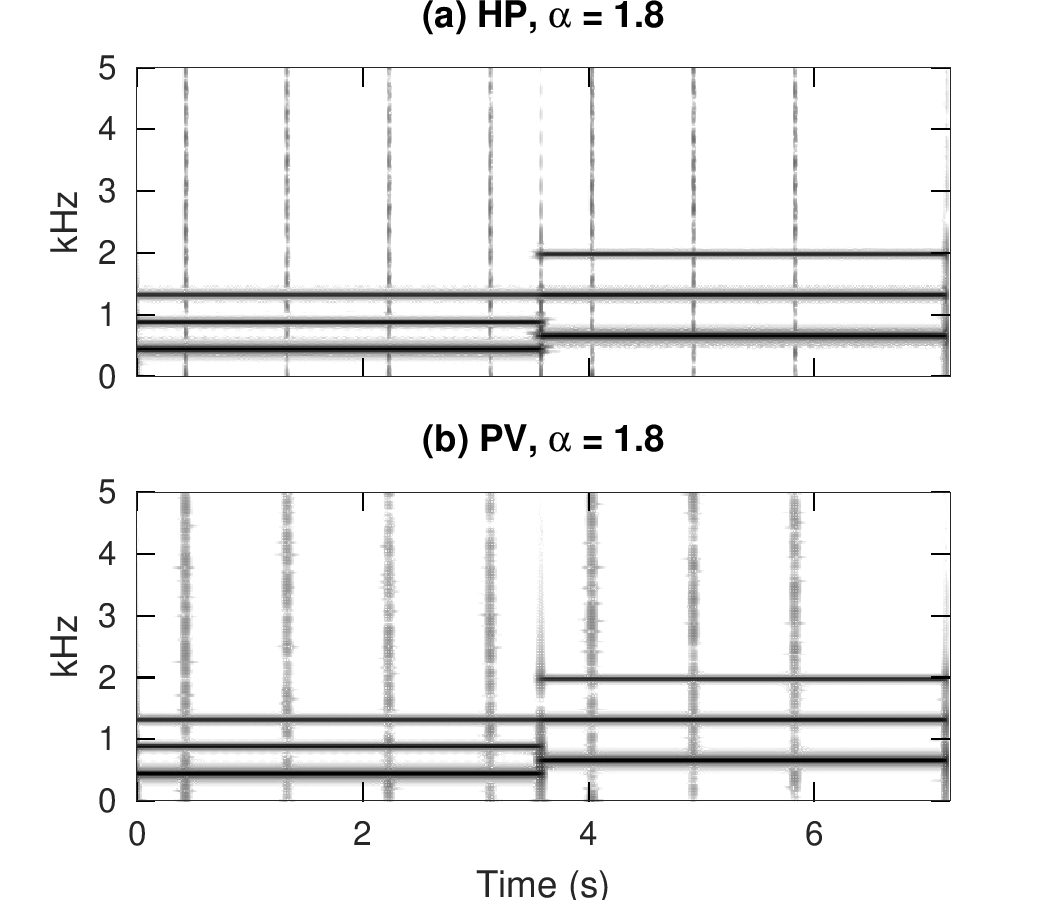
\includegraphics[width=\columnwidth]{fig/spec_hp_pv.png}
\caption{Spectrograms of the test mix stretched by $\alpha=1.8$. (a) HP: clicks remain thin vertical lines. (b) PV: clicks are smeared in time.}
\label{fig:spec}
\end{figure}

\subsection{Real music}
We also stretched an excerpt of \fillin{song title, artist}, a \fillin{genre / instruments} recording, \fillin{8} s long, by $\alpha=1.8$ with all four methods. \fillin{Number} listeners rated each version on the five-point scale of~\cite{driedger14} (1 = bad, 5 = excellent) after hearing the original. Table~\ref{tab:music} gives the results.

\begin{table}[t]
\centering
\caption{Real music excerpt, $\alpha=1.8$: mean opinion score}
\label{tab:music}
\begin{tabular}{@{}lcl@{}}
\toprule
Method & MOS & What listeners noticed \\
\midrule
HP & \fillin{--} & \fillin{} \\
PV & \fillin{--} & \fillin{} \\
WSOLA & \fillin{--} & \fillin{} \\
OLA & \fillin{--} & \fillin{} \\
\bottomrule
\end{tabular}
\end{table}

For comparison, the original paper, with 22 listeners and ten excerpts, reports average scores of 3.85 (HP), 2.89 (PV) and 2.44 (WSOLA) at $\alpha=1.2$, and 3.37, 2.24 and 1.90 at $\alpha=1.8$~\cite{driedger14}. \fillin{One sentence: do our scores show the same ranking? If not, why (clip choice, number of listeners)?}

\subsection{Runtime}
Table~\ref{tab:runtime} gives the processing time per minute of audio. \fillin{Re-measure in MATLAB with exp\_run\_all and replace these values.} HP costs roughly the PV plus the separation; the paper reports 4~s and 5~s per minute for its MATLAB implementation at $\alpha=1.2$ and $1.8$~\cite{driedger14}. Our version is slower, plausibly because our STFT loops over frames rather than being vectorised.

\begin{table}[t]
\centering
\caption{Seconds of processing per minute of audio}
\label{tab:runtime}
\begin{tabular}{@{}lcc@{}}
\toprule
Method & $\alpha=1.2$ & $\alpha=1.8$ \\
\midrule
HP & 7.4 & 10.0 \\
PV & 4.6 & 5.6 \\
WSOLA & 10.6 & 15.8 \\
OLA & 0.3 & 0.4 \\
\bottomrule
\end{tabular}
\end{table}

%======================================================================
\section{Discussion and Limitations}
\label{sec:discussion}

Our results reproduce the paper's central claim on controlled signals: splitting first lets the PV keep tones clean while short-frame OLA keeps transients crisp, without any transient detector. The method has known weaknesses. A singing voice is neither clearly harmonic nor clearly percussive, so much of it is assigned to the percussive part, and OLA's phase jumps then become audible; the paper finds that the plain PV beats HP on its singing excerpt~\cite{driedger14}. \fillin{Did your real-music clip show this? One sentence.} The PV also leaves some phasiness on sustained solo sounds, which identity locking reduces but does not remove~\cite{laroche99}.

Our evaluation is limited: the objective results use synthetic signals, the listening test is small, and we do not compare against the commercial \'elastique algorithm or the transient-handling method of Nagel and Walther~\cite{nagel09} used in the paper. Our hop sizes and WSOLA parameters are our own choices.

%======================================================================
\section{Conclusion}
We re-implemented harmonic--percussive time-scale modification in MATLAB from our own STFT upward, with the phase vocoder and WSOLA as baselines, and verified every block with unit tests. On a controlled test signal the method keeps clicks exactly as sharp as the original while the phase vocoder smears them. Future work includes a larger listening test on varied music, studying the separation's frame size $N$ and filter length $\ell$, which the paper also leaves open, and handling sounds such as the voice that are neither clearly harmonic nor percussive.

\section*{Author Contributions}
Anshika implemented and tested the harmonic--percussive separation. Mridhula implemented and tested the phase vocoder with identity phase locking. Anya Maheshwari implemented OLA and WSOLA, integrated the blocks and ran the experiments. All authors wrote the report.

\section*{Acknowledgment}
We thank Prof.~Vijay for guidance on the choice of paper and the project.

\begin{thebibliography}{8}

\bibitem{driedger14}
J.~Driedger, M.~M\"uller, and S.~Ewert, ``Improving time-scale modification of music signals using harmonic-percussive separation,'' \emph{IEEE Signal Process. Lett.}, vol.~21, no.~1, pp.~105--109, Jan. 2014.

\bibitem{flanagan66}
J.~L. Flanagan and R.~M. Golden, ``Phase vocoder,'' \emph{Bell Syst. Tech. J.}, vol.~45, pp.~1493--1509, 1966.

\bibitem{verhelst93}
W.~Verhelst and M.~Roelands, ``An overlap-add technique based on waveform similarity ({WSOLA}) for high quality time-scale modification of speech,'' in \emph{Proc. IEEE ICASSP}, Minneapolis, MN, USA, 1993.

\bibitem{nagel09}
F.~Nagel and A.~Walther, ``A novel transient handling scheme for time stretching algorithms,'' in \emph{Proc. 127th Audio Eng. Soc. Conv.}, New York, NY, USA, 2009, pp.~185--192.

\bibitem{fitzgerald10}
D.~Fitzgerald, ``Harmonic/percussive separation using median filtering,'' in \emph{Proc. Int. Conf. Digital Audio Effects (DAFx)}, Graz, Austria, 2010, pp.~246--253.

\bibitem{laroche99}
J.~Laroche and M.~Dolson, ``Improved phase vocoder time-scale modification of audio,'' \emph{IEEE Trans. Speech Audio Process.}, vol.~7, no.~3, pp.~323--332, 1999.

\bibitem{griffin84}
D.~W. Griffin and J.~S. Lim, ``Signal estimation from modified short-time Fourier transform,'' \emph{IEEE Trans. Acoust., Speech, Signal Process.}, vol.~32, no.~2, pp.~236--243, 1984.

\end{thebibliography}

\end{document}
